\documentclass[12pt]{exam}
\usepackage[portuguese]{babel}
\usepackage[utf8]{inputenc}
\usepackage{graphicx}
\usepackage{pdfpages}
% Please add the following required packages to your document preamble:
\usepackage{booktabs}

\graphicspath{{figuras/}}

\usepackage[margin=1in]{geometry}
\usepackage{amsmath,amssymb}
\usepackage{multicol}
\usepackage{textcomp,lmodern,listings}
\lstset{language=SQL,basicstyle=\ttfamily, columns=fullflexible, upquote, morekeywords={data,wrapper,library,language}}

\newcommand{\disciplina}{Banco de Dados}
\newcommand{\class}{\disciplina}
\newcommand{\term}{Professor: Igor Avila Pereira}
\newcommand{\bimestre}{2}
\newcommand{\valor}{4}
\newcommand{\examnum}{Atividade Avaliada - \bimestreº Bim. - Valor: \valor}
%\newcommand{\examdate}{xx}
%\newcommand{\timelimit}{4 horas}

\pagestyle{head}
\firstpageheader{}{}{}
\runningheader{\class} - {Página \thepage\ de \numpages}
\runningheadrule


\begin{document}

\noindent
\begin{tabular*}{\textwidth}{l @{\extracolsep{\fill}} r @{\extracolsep{6pt}} l}
\textbf{\class} & \textbf{Nome:} & \makebox[2in]{\hrulefill}   \\
\textbf{\examnum} & \textbf{Matrícula:} & \makebox[2in]{\hrulefill}   \\
%\textbf{\examnum} &&\\
%\textbf{\examdate} &&\\
\textbf{\term} &&\\
%\textbf{Duração: \timelimit}
\end{tabular*}\\
\rule[2ex]{\textwidth}{2pt}
\noindent
%rule[2ex]{\textwidth}{2pt}

\begin{questions}


\question (1.0) Implemente no SGBD PostgreSQL o Banco de Dados projetado pelo Modelo Relacional abaixo: 

\vspace{2px}

\textbf{Dicas:} CREATE SCHEMA, SET search\underline{\hspace{0.3cm}}path TO;
% \begin{itemize}
%     \item \textbf{Obs:} respeite nomes de tabelas/colunas/schemas, restrições de integridade e definição de schemas.
% \end{itemize}

\begin{figure}[!htp]
\centering
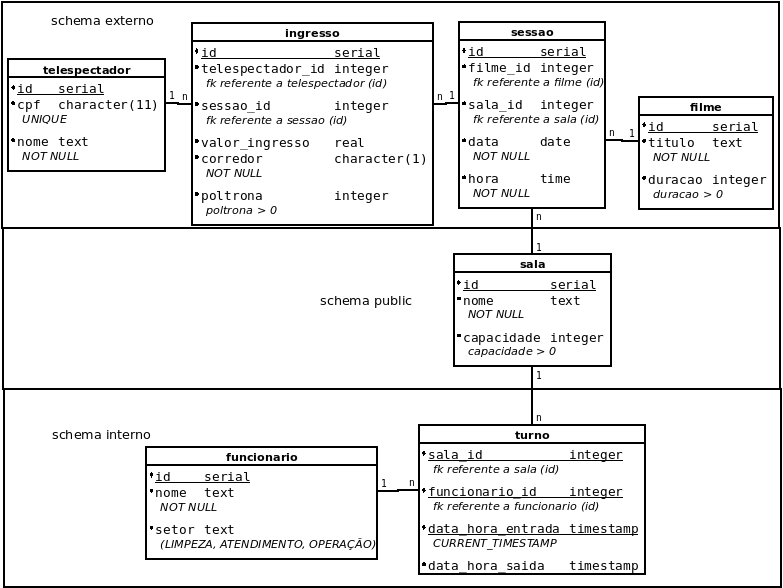
\includegraphics[width=1\linewidth]{figuras/prova1-2bim_2022.png}
\end{figure}



\question (0.5) Construa um STORE PROCEDURE de validação para a coluna \textit{cpf} da tabela \textbf{telespectador}.

\vspace{2px}

 \textbf{Observações:}

    \begin{itemize}
        \item Será preciso acrescentar o STORE PROCEDURE de validação à cláusula (\textit{check}) da coluna \textit{cpf} (tabela \textbf{telespectador});
    \end{itemize}

\textbf{Dicas:}

    \begin{itemize}
   \item A função desenvolvida nas aulas pode ser usada. Se não possuir a função em mãos, será preciso implementá-la novamente.
   
   \item Lembrando que 00000000000, 11111111111, 22222222222, 33333333333, 44444444444, 55555555555, 66666666666, 77777777777, 88888888888 e 99999999999 também são cpf's \textbf{INVÁLIDOS};
  \end{itemize}
  
\question (1.0) Sabendo que os Funcionários realizam diversos turnos, construa um STORED PROCEDURE que calcule o salário de um determinado funcionário mediante o número de horas trabalhadas por ele durante o mês atual (mês corrente). 

\vspace{2px}

\textbf{Observações:} 

\begin{itemize}
    \item Este STORED PROCEDURE deve ter como \textbf{parâmetros de entrada}: 
    \begin{itemize}
        \item o \textbf{id do funcionário} e,
        \item o \textbf{valor da hora trabalhada} de acordo com o seu setor:
        \begin{itemize}
\item Funcionários da \underline{\textbf{LIMPEZA}} ganham R\$ 10 por hora trabalhada,
\item Funcionários do \underline{\textbf{ATENDIMENTO}} ganham R\$ 15 e,
\item Funcionários da \underline{\textbf{OPERAÇÃO}} ganham R\$ 20.
\end{itemize}
    \end{itemize}
    \item Só vale turnos que começam e terminam no mesmo mês, ou seja, data\underline{\hspace{0.2cm}}hora\underline{\hspace{0.2cm}}entrada e data\underline{\hspace{0.2cm}}hora\underline{\hspace{0.2cm}}saida pertencem ao mesmo mês (mês atual);
\item Utilize os seguintes \textbf{casos de teste}: 
\begin{itemize}
    \item 1 funcionário de cada setor: LIMPEZA, ATENDIMENTO e OPERAÇÃO e,
    \item 2 turnos diferentes de trabalho para cada funcionário;
\end{itemize} 
\item \textbf{\underline{IMPORTANTE:}} Caso facilite o cálculo, é \textbf{permitido considerar somente horas inteiras/completas de cada turno de trabalho}: 
\begin{itemize}
    \item \textbf{Ex:} 
    \begin{enumerate}
        \item Em um turno que durou 3 horas, 30 minutos e 45 segundos, é permitido considerar somente 3 horas.
        \item Em um turno de 04:59, é permitido considerar somente 4 horas.
    \end{enumerate}
\end{itemize}
\end{itemize}

\textbf{Dicas:} EXTRACT, FOR LOOP, CAST e etc.

\question (1.0) Construa uma TRIGGER que, a cada novo funcionário, crie um novo turno de trabalho para este funcionário recém cadastrado.

\vspace{2px}

\textbf{Observações:}

\begin{itemize}
    \item 
    Este novo turno de trabalho deve começar no dia seguinte ao dia atual do cadastramento/inserção e deve começar às 08:00 (oito da manhã).
\item A sala onde este funcionário irá trabalhar em seu primeiro turno de trabalho deve ser escolhida aleatoriamente entre as salas existentes, ou seja, pela TRIGGER. 
% \item \textbf{Obs:} Os tipos das colunas da tabela \textbf{funcionario\underline{\hspace{0.3cm}}sala} (que representa o turno de trabalho) não devem ser alterados.
\end{itemize}

\textbf{Dicas:} ORDER BY RANDOM(), LIMIT, CURRENT\underline{\hspace{0.3cm}}DATE + INTERVAL '1 day'.

\question (0.5) Construa uma \textit{view} que retorne o \textbf{nome da sala}, o \textbf{título do filme}, o \textbf{nome do telespectador}, a \textbf{data} e \textbf{hora} da sessão, o \textbf{corredor} e a \textbf{poltrona} escolhida por cada telespectador para todos os ingressos. \textbf{Obs:} retornar \textbf{data} no formato dd/mm/aaaa.

% Ex:

% \begin{table}[]
% \begin{tabular}{@{}|c|c|c|c|c|c|c|@{}}
% \toprule
% \textbf{sala\_nome} & filme\_titulo & \textbf{telespectador\_nome} & \textbf{data} & \textbf{hora} & \textbf{corredor} & \textbf{poltrona} \\ \midrule
% 4k                  & TOP GUN       & igor                         & 2022-06-03    & 08:00         & A                 & 1                 \\ \midrule
% 4k                  & TOP GUN       & betito                       & 2022-06-03    & 08:00         & B                 & 15                \\ \bottomrule
% \end{tabular}
% \end{table}

\vspace{2px}

\textbf{Dicas:} CREATE VIEW, INNER JOIN.

\end{questions}


\includepdf[pages=-]{material/regra-cpf.pdf}

\end{document}